\section{Rendszerkövetelmények}

\subsection{Funkcionális és nem-funkcionális követelmények}

\indent Az alkalmazás fejlesztésének egyik legfontosabb kiindulópontja a világos és egyértelmű követelményrendszer meghatározása. A követelmények két fő kategóriába sorolhatók: funkcionális és nem-funkcionális követelmények. 

\subsection{Funkcionális követelmények}

A funkcionális követelmények azokat az elvárt viselkedéseket és szolgáltatásokat írják le, amelyeket a rendszernek teljesítenie kell. Ide tartoznak például a felhasználók által végrehajtható műveletek, az adatfolyamatok, valamint a rendszer reakciói különféle eseményekre vagy bemenetekre. A funkcionális követelmények meghatározzák, hogy mit csinál a rendszer, és ezek képezik az alapját a fejlesztési és tesztelési folyamatoknak.


\subsubsection{Contact}

A \textit{Contact} modell az alkalmazás felhasználóit reprezentálja, és lehetővé teszi a regisztráció, bejelentkezés, valamint a felhasználói adatok kezelésének funkcióit. A rendszer támogatja különböző szerepkörök (utas, sofőr, adminisztrátor) hozzárendelését a felhasználókhoz, amely szerepek befolyásolják a hozzáférési jogosultságokat. A felhasználók személyes adatai – beleértve a nevet, lakcímet és irányítószámot – utólag is módosíthatók a profilkezelő felületen keresztül. Az adminisztrátor jogosult egyes felhasználók inaktiválására is, amely funkció különösen hasznos a visszaélések vagy szabálytalanságok esetén történő fiókletiltás során.

\subsubsection{Ticket}

A \textit{Ticket} entitás a rendszerben megvásárolt jegyeket írja le, és szoros kapcsolatban áll a menetrendi adatokkal, valamint a felhasználói profillal. Jegyvásárlás során a rendszer automatikusan hozzárendel egy szabad ülőhelyet a kiválasztott járathoz. A tranzakció befejeztével a felhasználó egy automatikusan generált visszaigazoló e-mailt kap, amelyhez mellékletként QR-kód is csatolásra kerül.

Ez a QR-kód hordozza a legfontosabb utazási információkat, például a járatszámot, az indulási és érkezési állomásokat, valamint az útvonal teljes menetidejét. A felhasználó ezenkívül a \textit{Ticket Detail} nézeten keresztül részletesen is megtekintheti a jegyhez kapcsolódó adatokat – ideértve az indulás és érkezés időpontját, az utazási vonalat, valamint a kijelölt ülőhelyet.

A felület egy interaktív térképet is tartalmaz, amely grafikus formában mutatja be az adott utazás útvonalát. Fontos megjegyezni, hogy a QR-kód nem a jegyoldalon jelenik meg, hanem kizárólag a visszaigazoló e-mail mellékleteként kerül továbbításra, biztonsági és technikai okokból, közvetlenül a rendszer által generálva az aktuális jegyadatok alapján.

\subsubsection{Schedule}

A \textit{Schedule} entitás a menetrendi adatokat reprezentálja, különös tekintettel az indulási és érkezési időpontokra. Minden menetrendi egységhez pontos időkeretek társulnak, amelyek meghatározzák az adott járat működési időszakát. A rendszer automatikusan követi és frissíti az adott menetrendhez tartozó, még elérhető jegyek számát, figyelembe véve a korábban lezajlott foglalásokat és vásárlásokat. Ezen felül egy adott menetrendi bejegyzéshez egy konkrét buszjármű és egy előre definiált útvonal rendelhető hozzá, ami lehetővé teszi a teljes szállítási folyamat pontos és átlátható leképezését.

\subsubsection{TransportRoute}

A \textit{TransportRoute} entitás az alkalmazás központi elemei közé tartozik, mivel ez határozza meg a járatok által bejárt útvonalakat. Az adminisztrátorok számára biztosított funkciók segítségével új útvonalak hozhatók létre, a meglévők pedig módosíthatók vagy – szükség esetén – törölhetők a rendszerből. Minden útvonalhoz hozzárendelhetők meghatározott megállók, melyeket sorrendi információval is ellát a rendszer, lehetővé téve az útvonal pontos struktúrájának meghatározását.

\subsubsection{RouteStop}

A \textit{RouteStop} modell biztosítja az útvonalak és megállók közötti kapcsolat strukturált tárolását. Egy adott útvonalhoz tetszőleges számú megálló rendelhető, amelyek sorrendje kulcsfontosságú az útvonal logikája szempontjából. A rendszer minden kapcsolathoz egy egyedi sorrendértéket – úgynevezett \textit{SequenceNumber}-t – tárol, amely lehetővé teszi a megállók egymáshoz viszonyított elhelyezkedésének egyértelmű meghatározását.

\subsubsection{Stop}

A \textit{Stop} entitás a rendszerben nyilvántartott megállóhelyeket tartalmazza, beleértve azok megnevezését és földrajzi koordinátáit (GPS-alapú helymeghatározás). Ezek az adatok lehetővé teszik a megállók pontos térképes megjelenítését. A felhasználói élmény növelése érdekében a rendszer a Leaflet könyvtárat használja az interaktív térképes vizualizációhoz, amely dinamikusan mutatja az egyes megállók elhelyezkedését a térképen.

\subsubsection{Bus}

A \textit{Bus} modell a járműpark adatainak kezelésére szolgál. Minden egyes buszhoz rögzítésre kerül annak azonosító száma, befogadóképessége, típusa, valamint opcionálisan kép is társítható, amely vizuális információt nyújt az adott járműről. Egy busz több különböző menetrendhez is hozzárendelhető, lehetővé téve annak újrahasznosítását különböző időintervallumokban. Ezen túlmenően csatolmányok is kapcsolhatók a buszokhoz, például dokumentációk vagy karbantartási naplók.

\subsubsection{Attachment}

Az \textit{Attachment} entitás lehetőséget biztosít fájlok feltöltésére, amelyek kapcsolódhatnak buszokhoz vagy felhasználókhoz. A csatolmányok tárolása során megadható egy lejárati dátum is, amelynek segítségével szabályozható a fájlok érvényességi ideje. Ez a funkció különösen hasznos időszakos dokumentumok, például igazolások vagy engedélyek esetén, amelyek adott idő után automatikusan érvénytelenné válhatnak.

\subsubsection{AdminMessage}

A \textit{AdminMessage} modul lehetővé teszi, hogy a rendszer felhasználói közvetlen üzenetet küldjenek az adminisztrátorok számára. Az elküldött üzenetek strukturált módon kerülnek eltárolásra a rendszerben, ahol minden bejegyzéshez tartozik egy olvasottsági státusz is. Ennek segítségével nyomon követhető, hogy az adott kérdés vagy észrevétel feldolgozásra került-e már az adminisztrációs oldalról.

\subsubsection{AdminTask}

Az \textit{AdminTask} komponens célja az adminisztrátori feladatok rendszerezett kezelése. A rendszer lehetőséget biztosít új feladatok létrehozására, amelyekhez megadható egy szöveges leírás, valamint egy határidő is. A feladatok státusza dinamikusan módosítható, jelezve, hogy azok már megoldásra kerültek-e, vagy még folyamatban vannak. Ez a modul hatékony eszközként szolgál az adminisztratív munkafolyamatok menedzselésében.



\subsection{Nem-funkcionális követelmények}

A nem-funkcionális követelmények a rendszer minőségi jellemzőit írják le. Ezek nem konkrét műveleteket határoznak meg, hanem a működés módjára, körülményeire, illetve elvárt teljesítményére vonatkoznak. Ilyenek például a válaszidő, a rendelkezésre állás, a biztonság, a skálázhatóság vagy a felhasználói élmény. Bár ezek nem közvetlenül kapcsolódnak az egyes funkciókhoz, a végfelhasználói elégedettség és a rendszer hosszú távú fenntarthatósága szempontjából kiemelten fontosak.

\subsubsection{Elérhetőség és platformfüggetlenség}

A rendszer webböngészőn keresztül érhető el, elsősorban laptopokon és asztali számítógépeken való használatra optimalizálva. Mobiltelefonokon és táblagépeken való megjelenítés jelenleg nem támogatott, mivel a felhasználói felület elrendezése és interakciói kifejezetten nagyobb képernyőkre lettek tervezve.

\subsubsection{Aszinkron működés szerepe}

\indent A rendszer működésének optimalizálása érdekében kiemelt figyelmet kapott az aszinkron feldolgozás alkalmazása. Ez a megközelítés lehetővé teszi, hogy a különböző háttérfolyamatok – például adatfeldolgozás vagy külső szolgáltatásokhoz történő kapcsolódás – ne akadályozzák a felhasználói felület zökkenőmentes működését. Azáltal, hogy a műveletek nem blokkolják egymást, biztosítható a gyors válaszidő és a gördülékeny felhasználói élmény. Az aszinkron logika tehát jelentős szerepet játszik abban, hogy a rendszer egyidejűleg több feladatot is képes hatékonyan kezelni, ezáltal növelve az alkalmazás általános teljesítményét és megbízhatóságát.


\subsubsection{Biztonság}

A felhasználók adatainak védelme kiemelt prioritás. Az alkalmazás SSL titkosítással biztosítja a hálózaton történő adatátvitel biztonságát. A jelszavakat és más érzékeny információkat erős titkosítási algoritmusokkal tárolja a rendszer. A különböző szerepkörökhöz (pl. adminisztrátor, utas) eltérő jogosultsági szintek tartoznak, és az adminisztratív funkciók kizárólag megfelelő jogosultság birtokában érhetők el. Inaktivitás esetén a rendszer automatikusan kijelentkezteti a felhasználót, ezzel csökkentve az illetéktelen hozzáférés kockázatát.

\subsubsection{Felhasználói élmény (UX)}

A felhasználói felület kialakításakor a könnyű kezelhetőség és az átláthatóság volt a fő szempont. A navigáció logikus szerkezetet követ, a funkciók koherens sorrendben jelennek meg. A rendszer egyértelmű vizuális visszajelzéseket biztosít minden felhasználói művelet során, segítve ezzel az interakciók megértését. A gombok és menüpontok érthető, leíró feliratokkal rendelkeznek. A térképes útvonalmegjelenítés jól olvasható, vizuálisan is könnyen követhető formában történik, ami különösen fontos az utazástervezés során.

\subsubsection{Skálázhatóság és karbantarthatóság}

A rendszer kialakítása moduláris, így új funkciók vagy komponensek későbbi hozzáadása különösebb átalakítás nélkül megvalósítható. A forráskód fejlesztése során a SOLID alapelvek és a Clean Code gyakorlat került alkalmazásra, ezáltal biztosítva a kód hosszú távú karbantarthatóságát. A fejlesztés verziókezelő rendszerrel (pl. Git) történik, amely támogatja a kollaboratív munkát és a változások visszakövethetőségét. A rendszer eseménynaplózással követi a fontosabb műveleteket és hibákat, elősegítve ezzel a megbízható üzemeltetést és a gyors hibaelhárítást.

\subsubsection{Technológiai megfelelés}

A rendszer fejlesztése a korszerű ASP.NET Core MVC keretrendszerre épül, amely biztosítja a modern webalkalmazásokhoz szükséges architektúrát és teljesítményt. A fejlesztési környezet legalább .NET 6-os verzióra épül, amely támogatja a legújabb nyelvi és futtatási fejlesztéseket. A térképes megjelenítés a Leaflet JavaScript könyvtár segítségével történik, amely egy könnyű és bővíthető eszköz interaktív térképek készítésére.

\newpage
\subsection{Használati esetek és felhasználói szerepkörök}

A rendszer három jól elkülöníthető felhasználói szerepkört különböztet meg, melyek mindegyike eltérő jogosultságokkal és funkcionalitással rendelkezik. Ez a szerepköralapú hozzáférés lehetővé teszi, hogy minden felhasználó kizárólag az általa betöltött pozícióhoz szükséges műveleteket végezhesse el, ezzel is elősegítve a biztonságos és strukturált rendszerhasználatot.

Az adminisztrátori szerepkörrel rendelkező felhasználók teljes körű hozzáféréssel bírnak a rendszer valamennyi komponenséhez. Ők felelnek a felhasználói fiókok kezeléséért, szerepkörök és jogosultságok beállításáért, továbbá a működéshez szükséges konfigurációk elvégzéséért. Emellett az adminok felügyelik az útvonalakat, menetrendeket, valamint rendszeres jelentéseket készítenek a működés hatékonyságáról. Az adminisztrátori jogosultságok biztosítják a hibakezeléshez, rendszeresemények nyomon követéséhez és az általános üzemeltetéshez szükséges eszközöket is.

\begin{figure}[h!]
    \centering
    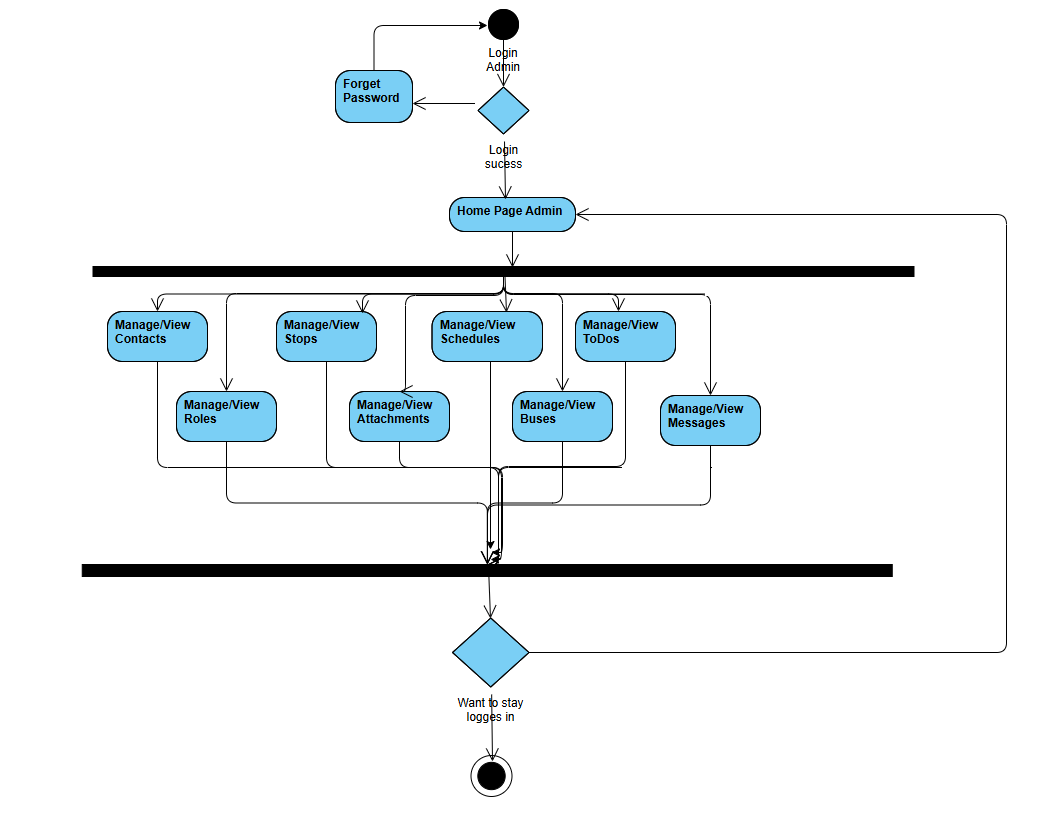
\includegraphics[width=0.90\textwidth]{Szakdolgozat/Mellekletek/activityadmin.PNG}
    \caption{Az adminisztrátor rendszerhasználata: bejelentkezés után útvonalak és menetrendek kezelése, riportok készítése, valamint felhasználói jogosultságok beállítása.}
    \label{fig:admin-activity}
\end{figure}

A második csoportot a külső felhasználók alkotják, akik jellemzően ügyfelek vagy utasok, és csak a saját adataik kezelésére kapnak jogosultságot. Számukra a rendszer lehetőséget nyújt a személyes adatok megtekintésére és frissítésére, jegyek foglalására és kezelésére, valamint különböző rendszerértesítések – például státuszváltozások vagy foglalási visszaigazolások – fogadására. Amennyiben problémát észlelnek, ők is jelezhetik azt az ügyfélszolgálat felé, ezzel támogatva a szolgáltatásminőség fenntartását.

\begin{figure}[h!]
    \centering
    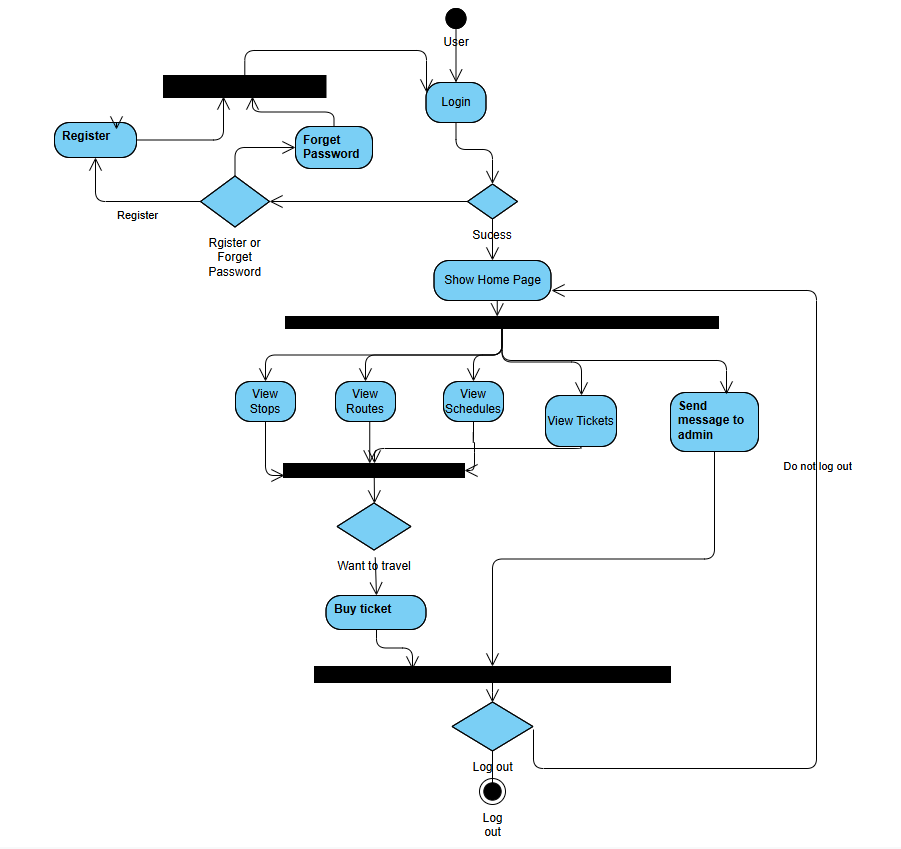
\includegraphics[width=0.85\textwidth]{Szakdolgozat/Mellekletek/activityuser.PNG}
    \caption{A felhasználó bejelentkezés utáni tevékenységeinek folyamata: megállók megtekintése, jegyfoglalás, üzenetküldés, valamint a jegyek áttekintése.}
    \label{fig:user-activity}
\end{figure}

A fentiek alapján megállapítható, hogy a szerepkörök világos elhatárolása lehetővé teszi a felhasználók számára, hogy csak az általuk végzendő feladatokhoz szükséges funkciókat érjék el. Ez nemcsak a kezelhetőséget javítja, hanem jelentősen növeli a rendszer biztonságát és megbízhatóságát is.





